\section{Estimation}\label{sec:estimation}

The calibrator, called J, maximises the likelihood of Section~\ref{sec:likelihood} over $\theta=(\eta,\beta,\eps,\kappa)$ and
reports, for each parameter, a profile-likelihood interval and the claim that the interval supports. Variants add an
external hazard and a fit window (H), pin $\kappa$ (kfix), fit a window without a hazard with profile intervals (W), or fit a
window without a hazard by an earlier envelope method (W0). All pseudocode is in SI
Section~\ref{sec:si-algorithms}.

\paragraph{Seed and maximum likelihood.} Individuals are first prepared: the censoring-tie relabelling of
Section~\ref{sec:likelihood} is applied where its pattern holds, and the grid is chosen. A deterministic least-squares fit to
the Kaplan--Meier curve gives a seed. The log-likelihood is then maximised in $z=\log\theta$ by bounded L-BFGS-B
\citep{byrd1995limited,zhu1997algorithm} on exact gradients from two starts, the seed and the seed with $\eps$ multiplied by
\C{m-eps-start}, and the better optimum is kept. The search box is [\C{m-box-lo},\,\C{m-box-hi}] for $\eta$, $\beta$ and $\eps$ in the time
unit of the data, and [\C{m-kappa-lo},\,\C{m-kappa-hi}] for $\kappa$ (the box in $\kappa$ is in units of the threshold). The upper edge of
$\kappa$ is a modelling choice: for $\kappa\gg1$ removal is linear in $x$ and $\beta$ and $\kappa$ trade off along a ridge, so an
upper end of raw $\beta$ may be set by the box and not by the data (Section~\ref{sec:identifiability}). Stopping tolerances and
iteration limits are in SI Table~\ref{tab:switches}.

\paragraph{Profile walks.} For each parameter $p$ the profile log-likelihood $\ell_p(v)=\max\ell(\theta)$ over the other
parameters with $\theta_p=v$ is evaluated at nodes placed by an adaptive walk outward from $\hat\theta_p$ on each side, in
$\log v$. The first step is \C{m-step0} decades and grows while the deviance $D=2[\ell(\hat\theta)-\ell_p(v)]$ changes slowly, up to
\C{m-step-max} decades; a step that makes $D$ jump by more than \C{m-dev-jump} is rejected and retried with the step divided by \C{m-step-shrink}. A side
stops at $D\ge\C{m-dev-stop}$, at the search box, or after \C{m-per-side} accepted nodes. Each node is a bounded L-BFGS-B solve over the other three
parameters, warm-started from the previous node, and restarted from the seed's values when it lands in a degenerate corner (for
example $\beta$ at its floor, which switches removal off). Three passes follow. \emph{Repair}: a node whose value is lower than
a node further out by more than \C{m-repair-nats} nats is re-solved from that node's solution, because a warm-start chain that stalls
once stays stalled. \emph{Polish}: the nodes that place the two interval edges, and the node just inside each, are re-solved from several
fresh starts (the optimum's nuisance values, the seed's, a neighbour's, and the opposite corners of $\kappa$); the edge moves
outward if the polished node now falls inside, at most \C{m-polish-moves} times per side. \emph{Bisection}: a crossing bracket wider than
\C{m-bisect-dex} decades is bisected, at most \C{m-bisect-max} times per side, so that an edge is not set by a coarse node.
Figure~\ref{fig:profile}A shows one walk on an illustrative profile, with the growing steps, a rejected step and the two
ways a side stops; Figure~\ref{fig:profile}B sketches the three passes.

\paragraph{Intervals.} The interval of $p$ is the set of $v$ with deviance below the $\chi^2_1$ quantile at level
\C{m-level}, $\C{m-chi2}$, i.e.\ within $\C{m-chi2-half}$ nats of the profile maximum \citep{venzon1988method,raue2009structural}. Its edges are the
first crossings outward from the outermost accepted nodes, interpolated linearly in $\sqrt D$ against $\log v$, which is exact for a
quadratic profile. Two safeguards guard against edges that are too narrow. First, \emph{self-consistency widening}: the
interval is extended to cover every point that the fit evaluated anywhere (in the maximisation, the walks, repair, polish) and
whose log-likelihood lies within $\C{m-chi2-half}$ nats of the best value found. Second, a \emph{basin re-fit}: if any profile node beats the
reported maximum by more than $\C{m-chi2-half}$ nats, the maximisation stopped in a wrong basin, and it is restarted from the best nodes and from a
ladder of larger $\eta$, all profiles are recomputed, and this is repeated at most \C{m-refit-max} times.
Figure~\ref{fig:profile}C shows the cut, the interpolated edges and a one-sided case on stored walks, and
Figure~\ref{fig:profile}D sketches the two safeguards.

\begin{figure}[p]
\centering
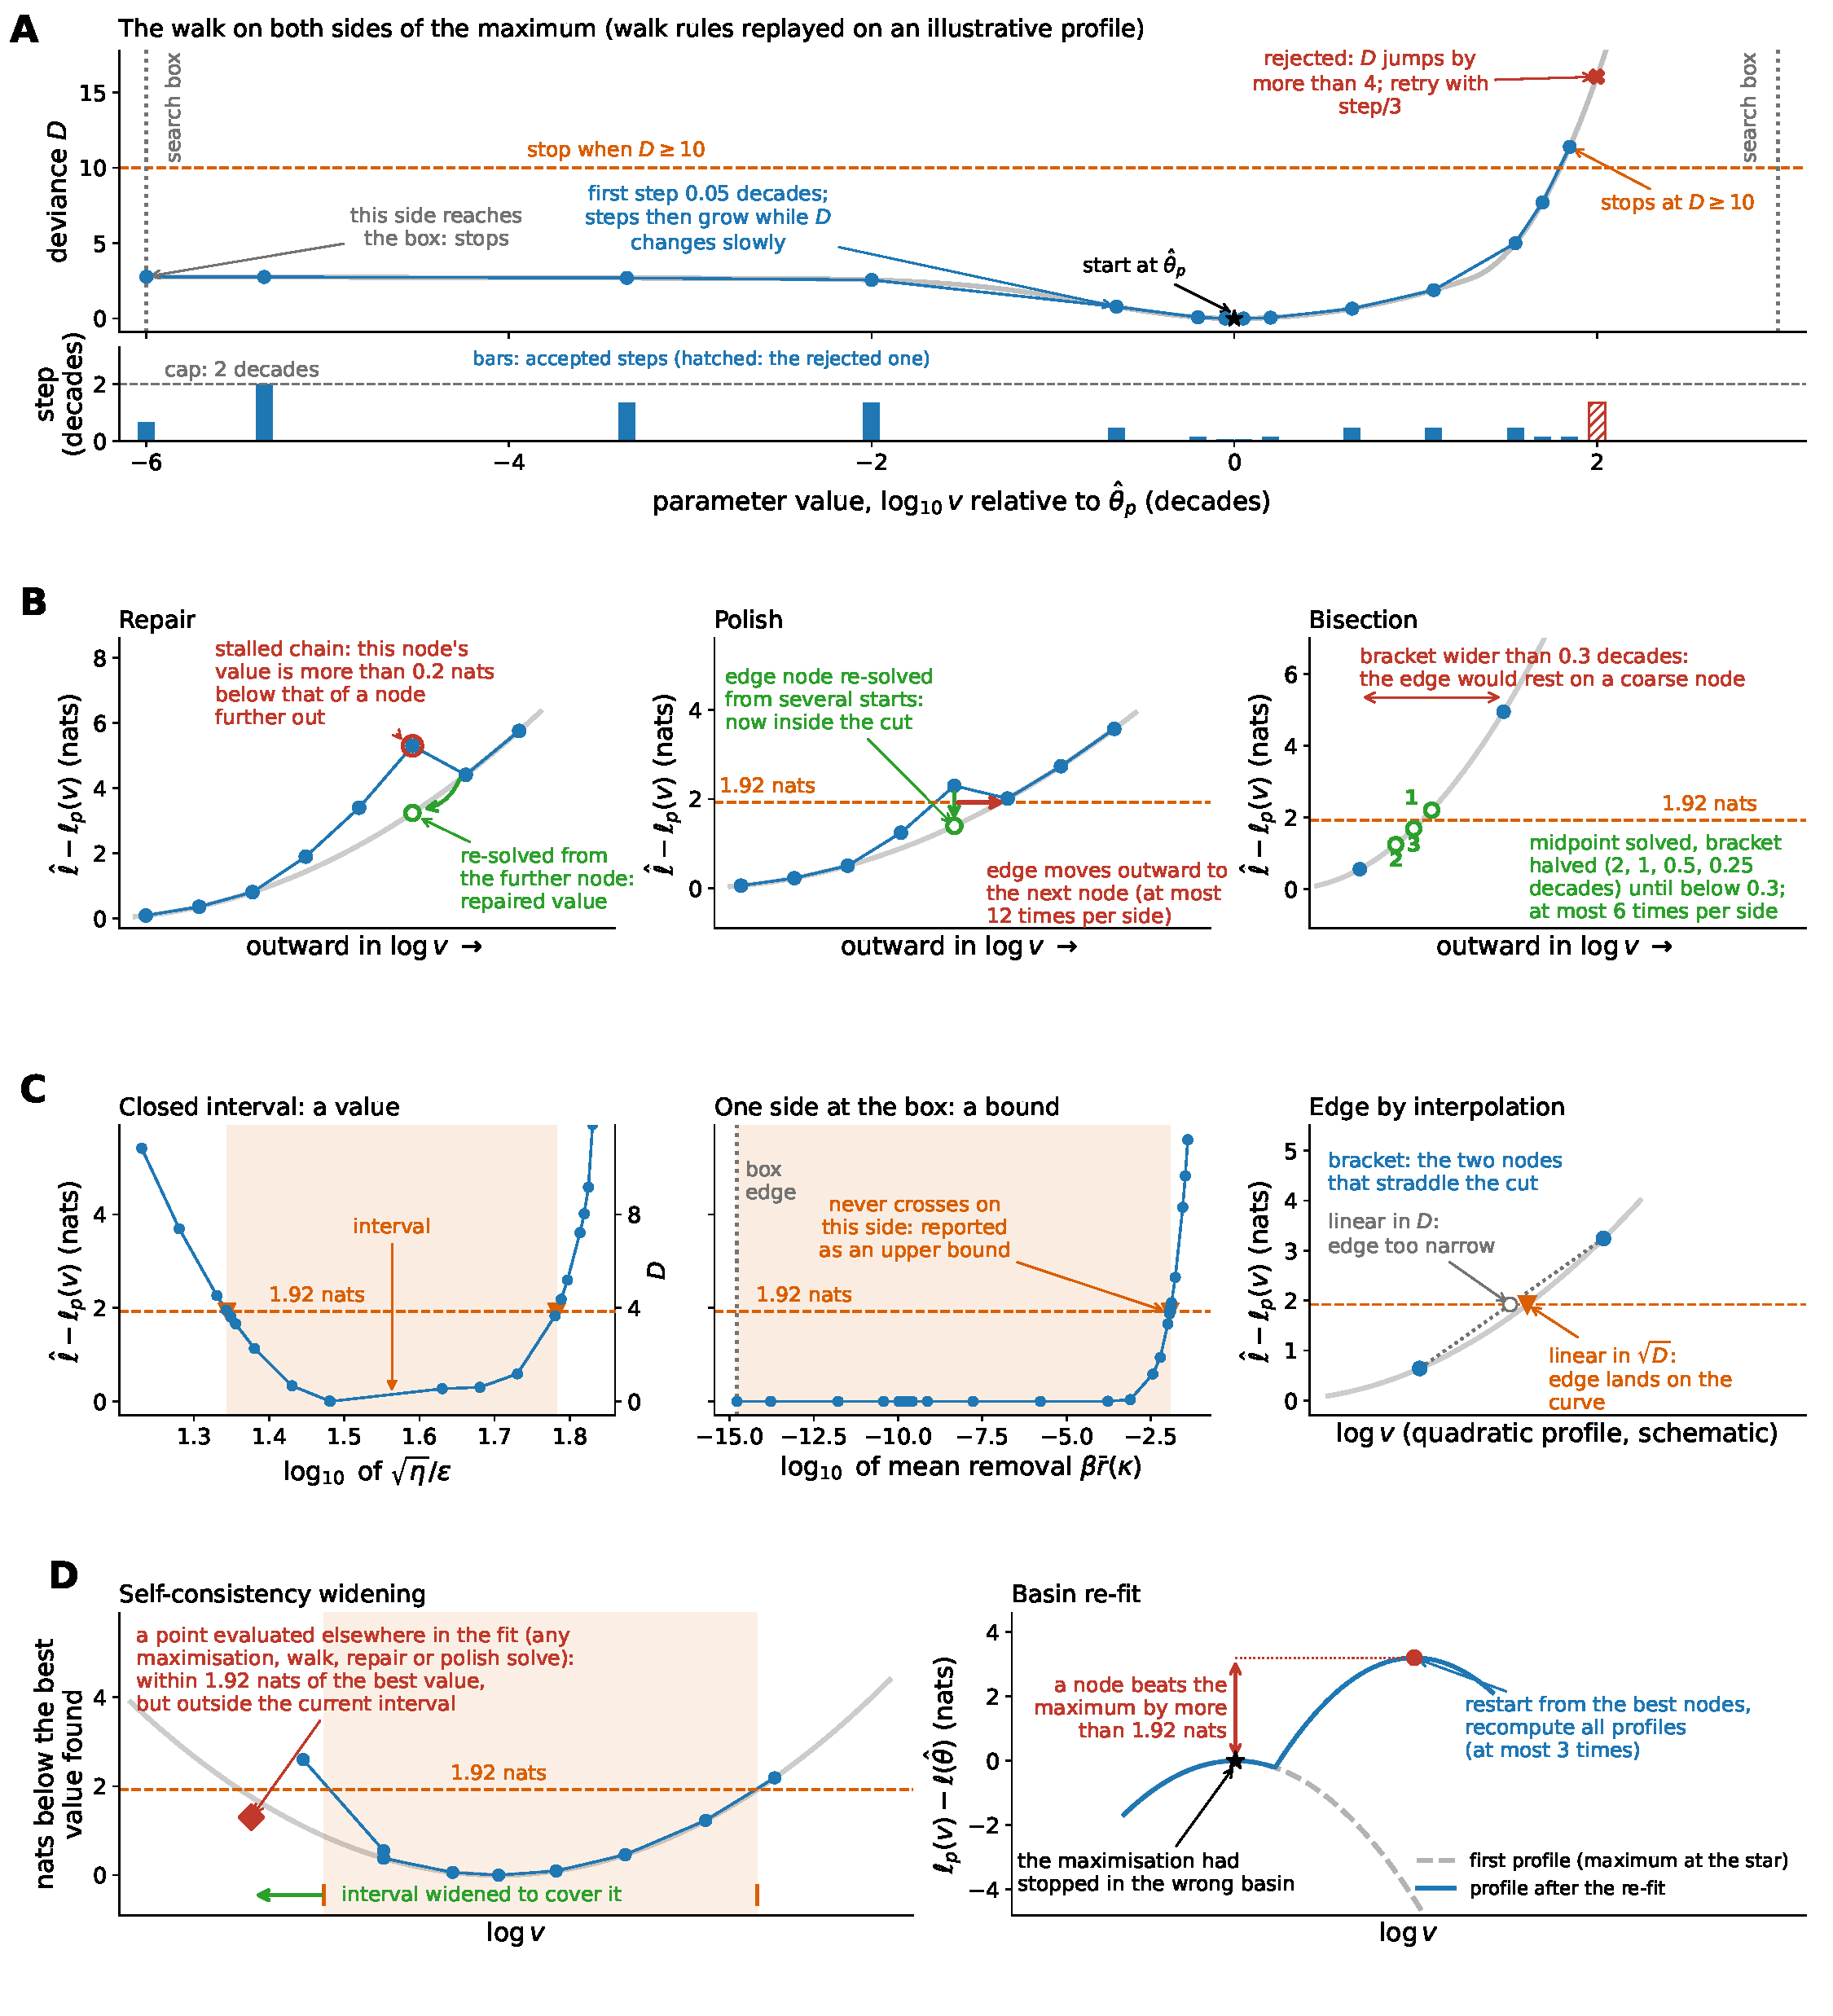
\includegraphics[width=0.64\textwidth]{fig_profile.pdf}
\caption{\textbf{How a profile is walked, repaired and turned into an interval.}
\textbf{A}, the walk on both sides of the maximum $\hat\theta_p$, in $\log_{10}v$. Blue dots are accepted nodes, the lower strip shows the
step taken to each. The first step is \C{m-step0} decades; it grows while $D$ changes slowly, up to \C{m-step-max} decades. A step that
raises $D$ by more than \C{m-dev-jump} is rejected (red cross, hatched bar) and retried with the step divided by \C{m-step-shrink}.
A side stops at $D\ge\C{m-dev-stop}$ (right) or at the search box (left).
\textbf{B}, the three passes that follow, shown as sketches. \emph{Repair}: a node whose value lies more than \C{m-repair-nats} nats below
that of a node further out is a stalled warm start; it is re-solved from the further node (green circle). \emph{Polish}: the node that places an
edge is re-solved from several starts; it now falls inside the cut, so the edge moves outward (at most \C{m-polish-moves} times per side).
\emph{Bisection}: a bracket wider than \C{m-bisect-dex} decades is halved by midpoint solves (numbered), at most \C{m-bisect-max} times per side.
\textbf{C}, from nodes to interval. Left: a closed interval, the set of $v$ within \C{m-chi2-half} nats of the maximum (shaded; right axis: $D$).
Middle: a profile that stays flat to the box on one side crosses the cut on the other only, so J reports a bound, not a value. Right: each edge is placed
by interpolating $\sqrt D$ linearly against $\log v$ between the two nodes that straddle the cut; this is exact for a quadratic profile, whereas
interpolating $D$ itself would place the edge too close to the maximum.
\textbf{D}, the two safeguards. Left: a point evaluated anywhere in the fit that lies within \C{m-chi2-half} nats of the best value but outside the interval
widens the interval to cover it. Right: a profile node that beats the reported maximum by more than \C{m-chi2-half} nats shows that the maximisation
stopped in a wrong basin; the fit restarts from the best nodes, recomputes all profiles, and repeats this at most \C{m-refit-max} times.
\emph{Real and illustrative parts.} C, left and middle, are stored walks of two benchmark cohorts
($\sqrt\eta/\varepsilon$ of \code{ratio-lo/cv-mid/n-10000}; $\beta\bar r(\kappa)$ of \code{ratio-lo/cv-broad/n-1000}), including the
nodes added by repair, polish and bisection. In A the step rules are replayed on an invented profile; B, C right and D are sketches.}
\label{fig:profile}
\end{figure}

\paragraph{From profile to claim.} The shape of each profile decides what J claims. A profile that crosses the cut on both
sides gives a \emph{value}: the closed interval. A profile that crosses on one side only gives a \emph{bound}, an upper
bound if only the upper end is finite and a lower bound otherwise. A profile that crosses on neither side, or has too few
finite nodes, gives \emph{no claim}. Ends are clipped to the search box, and the point reported with a claim is
$\hat\theta_p$. For $\kappa$ most profiles are flat: no claim was made for a fraction \C{v6-J-kappa-declined-frac} of the v6 benchmark
cohorts. Quantities that survival data do identify but that are not coordinates ($\sqrt\eta/\eps$, the mean removal
$\beta\,\rbar(\kappa)$) are claimed by profiling the quantity itself with the same walk, constrained to $\log g(z)=c$, rather
than by combining the intervals of the parameters.

\paragraph{Variants.}
\emph{H (external hazard and window).} H adds a constant external hazard $h$ as a fifth, nuisance coordinate in a box
[\C{m-h-lo}$/L$,\,\C{m-h-hi}$/L$] (units of the Kaplan--Meier mean lifetime), and accepts a fit window $[\mathrm{lo},\mathrm{hi})$ as in
Section~\ref{sec:likelihood}. Its extra starts are a Makeham curve fit and a ladder of hazard values; a second chain solves each
profile node with $h$ reset to its floor, so that H's profiles cannot fall below those of J on the same data. $h$ is never
reported: it is not a claimed quantity, it can trade off against removal, and only its effect on the other intervals is of
interest. On sharp cohorts with a hazard the likelihood grid can be off by up to \C{h-sharp-offset-max} nats (Section~\ref{sec:limitations}).

\emph{kfix ($\kappa$ pinned).} Because $\kappa$ is not identified, a variant fixes it at $\kappa_0$ and fits $(\eta,\beta,\eps)$ only.
The coordinate is masked (the parameter vector and all code paths are unchanged), the seed is mapped to $\kappa_0$ keeping
$\beta/(1+\kappa)$, and no profile of $\kappa$ is computed. We recommend $\kappa_0=\C{m-kappa0}$, for which removal is nearly zero-order
(saturated) over the whole damage range and $\rbar(\kappa_0)$ is close to one. kfix claims are conditional on $\kappa=\kappa_0$. It
claims $\eta$, $\eps$ and the identified $\sqrt\eta/\eps$ with the usual shapes, and $\beta$ at $\kappa_0$, which is not the
$\beta$ of the data-generating process unless that process also has $\kappa=\kappa_0$. Mean removal is therefore read as
$\beta\,\rbar(\kappa_0)$, never as $\beta/(1+\kappa)$. One run costs \C{kfix-J0001-cpu} of the total CPU of the $\kappa$-free fit on the benchmark's
medium tier. An H-kfix combines the two.

\emph{W (windowed calibrator, $h=0$).} W is the calibrator J with a fit window and no external hazard. It is
\code{sraging}'s composition of J 1.0.1 with the window switched on and the hazard switched off; no release of the calibrator
itself ran it. It maximises the likelihood of the observations inside the window $[\mathrm{lo},\mathrm{hi})$, conditioned on
survival to $\mathrm{lo}$ and censored at $\mathrm{hi}$ (Section~\ref{sec:likelihood}), and it uses J's profile walk, interval
widening and claim shapes unchanged. Without a window it returns exactly what J returns: every number of the fit was equal on
\C{w-id-nowin} cohorts. With a window it gives the same fit as the frozen 1.0.1 code run with the same switches
(\C{w-id-win-pairs} pairs of fits, W and H on two windowed cohorts). One effect of the window is common. A death recorded at
$\mathrm{hi}$ happened after the window closed, so it is censored at $\mathrm{hi}$; over the \C{w-edge-nfits} windowed fits of
the benchmark this censored a median of \C{w-edge-med}\,\% of a cohort's records and at most \C{w-edge-max}\,\%. An open window,
$\mathrm{hi}=\infty$, needs a recording interval $\delta$: $\mathrm{hi}$ is then set to the first grid point past the last record.
The window is one per cohort; per-individual entry ages are refused. Use W when the data cover only part of life and there is
no reason to add an external hazard: animals enrolled at an age, a life table that starts late, a study stopped before the last
deaths. Use H instead when an age-independent external hazard is part of the question. Use W rather than W0, because W has
profile intervals with claim shapes and a measured coverage (Section~\ref{sec:val-benchmark}). On the small and medium cohorts
where W and H both gave a closed claim whose upper end the data set, the two were about equally wide: the paired median of
$\log_{10}$(width of W / width of H) was \C{w-wh-eta-med} dex for $\eta$ (\C{w-wh-eta-n} cohorts) and \C{w-wh-eps-med} dex for
$\eps$ (\C{w-wh-eps-n}).

Read the upper ends of W's claims with care. On these windows $\eta$, $\eps$ and $\beta/\kappa$ slide together along a ridge
of the model that ends at the search box, so an upper end is often the box's and not the data's. Some upper ends were also stopped short by the
profile walk and then widened to points the fit had already evaluated. The claim label says which. An upper end labelled
\emph{box-limited} or \emph{edge not found} means ``at least this'', not the end of the interval. Use the lower ends. Read the
ratio $\eta/\eps$, which closed and covered the truth where $\eta$ alone stayed open; $\beta\rbar/\eta$ closed less often and was
otherwise an upper bound, which also covered the truth (Section~\ref{sec:val-benchmark}). Apply this at every sample size. For $n\ge\C{w-large-n}$ rows the software also warns, because
the large synthetic cohorts at human life tables showed most upper ends not set by the data; the warning is keyed to sample
size, but below that size the same life tables behave the same way, and the labels are then the only signal.

\emph{W0 (windowed engine fit, $h=0$).} W0 is the earlier envelope fit for the same case. It is the maximum-likelihood fit of
the model with $h=0$ on the windowed observations, conditioned on $S(\mathrm{lo})$ and censored at $\mathrm{hi}$, with the same
grid and likelihood as H. It is an engine fit rather than a calibrator run. The point estimate is the best of several bounded
L-BFGS-B fits from different starts (the null fit of a hazard test, a fit of the windowed data by J's model, and H's optimum with
$h$ set to zero), each with one jittered restart; it can be run with $\kappa$ free or pinned. W0 has no profile walk and no claim
shapes. Its intervals come from a likelihood envelope: the $(\beta,\kappa)$ plane is covered by a coarse grid; at each node
$\eta$ and $\eps$ are re-fitted; the direction in $(\log\eta,\log\eps)$ along which the likelihood is flattest is walked both
ways to a cut slightly beyond the nominal one; and the interval of any quantity is its range over the nodes whose log-likelihood
is within $\C{m-chi2-half}$ nats of the global maximum. The range over a finite set of nodes can be narrower than the profile
interval where nodes are sparse. W0's envelope intervals have not been scored against the truth, and W0 is project code, not
part of the released package. A study that used W0 should compare it with W on its own data, as in the bridge procedure of SI
Section~\ref{sec:versions}.

\paragraph{What the user supplies and receives.} The input is a vector of ages (in any time unit, used consistently, since the
box is in that unit), event flags (1 for death, 0 for censored), the recording resolution $\delta$, or a statement that times are
exact, and for H, W or W0 an optional window $[\mathrm{lo},\mathrm{hi})$. The output is the point estimate $\hat\theta$, a claim per
parameter (shape, ends, point), claims for the identified combinations, the log-likelihood, the grid that was used, and a set of
truth-free warnings: a profile that found a better point, a death on the numerical floor, a censoring tie, recording ages that
are not on the $\delta$ grid, an estimate on the upper edge of the box (Section~\ref{sec:software}).

\paragraph{Cost.} A fit evaluates the likelihood and its gradient thousands of times, since every profile node is itself an
optimisation. The cost below is CPU time per complete fit, that is, the maximum-likelihood search and all profile
intervals, read from the stored records of the benchmark runs (\C{fcost-J-n} cohorts for each of the calibrator J and its
external-hazard variant H; a third run of J adds the sharp cohorts). The median fit takes \C{fcost-J-median} CPU-seconds
(\C{fcost-J-med-min} minutes) for J, with a 90th percentile of \C{fcost-J-q90} (\C{fcost-J-q90-min} minutes) and a
maximum of \C{fcost-J-max} (\C{fcost-J-max-h} hours). H costs about twice as much: median \C{fcost-H-median}
(\C{fcost-H-med-min} minutes), maximum \C{fcost-H-max-h} hours. Cost rises with $n$ because the $N$ rule raises the grid:
of the J fits, \C{fcost-J-N900} used $N=900$, \C{fcost-J-N1800} used $1800$ and \C{fcost-J-N3600} used $3600$ cells, and
the median rises from \C{fcost-A-out-lt1e3-med} CPU-seconds below $10^3$ individuals to \C{fcost-A-out-5e4-med} above
$5\times10^4$ (Table~\ref{tab:fitcost}).

Sharp cohorts are the expensive case. Where the step rule applies ($\mathrm{CV}_c<0.05$), the median fit takes
\C{fcost-A-in-median} CPU-seconds (\C{fcost-A-in-med-h} hours; 90th percentile \C{fcost-A-in-q90-h} hours, maximum
\C{fcost-A-in-max-h}), against \C{fcost-A-out-median} (\C{fcost-A-out-med-min} minutes) for the other
\C{fcost-A-out-n} fits of the same run, a factor of \C{fcost-ratio-med}. The factor holds at matched $n$: for $10^3\le n<5\times10^3$ the
medians are \C{fcost-A-in-1e3-med} and \C{fcost-A-out-1e3-med} CPU-seconds. A user with a sharp cohort should therefore
expect hours, not minutes. Counted as CPU per likelihood or gradient evaluation (the whole fit's CPU divided by the number of
evaluations, so including start-up and the profile search), the J median is \C{fcost-eval-900}~ms at $N=900$,
\C{fcost-eval-1800}~ms at $N=1800$ and \C{fcost-eval-3600}~ms at $N=3600$. The records hold no timing of a single evaluation
(the stored MLE time covers only the first stage while the evaluation count covers the whole fit), so these are averages.

These are CPU seconds, not wall-clock time, and they were measured on a mixed cluster: \C{fcost-ncpu} CPU models
(Intel Xeon Gold 5320, 6230R and 6438Y+; AMD EPYC 9754 and 9634). Within J the median is \C{fcost-cpu-fast} CPU-seconds on EPYC 9754 and
\C{fcost-cpu-slow} on Xeon Gold 5320, so absolute times can differ by tens of percent with the host. The sharp-cohort
run did not control for host, and its cohorts overlap those of the main run.

\begin{table}[t]
\centering\small
\caption{CPU-seconds per complete fit by cohort size and sharpness (calibrator J, run with the sharp cohorts included), and
the median for the external-hazard variant H on the main cohort set. ``Sharp'' means the step rule applies ($\mathrm{CV}_c<0.05$).
Counts are fits; q90 is the 90th percentile. No sharp cohort has $n\ge2\times10^4$.}\label{tab:fitcost}
\begin{tabular}{@{}lrrrrrrr@{}}
\toprule
 & \multicolumn{3}{c}{not sharp} & \multicolumn{3}{c}{sharp} & H, median\\\cmidrule(lr){2-4}\cmidrule(lr){5-7}
$n$ & fits & median & q90 & fits & median & q90 & \\\midrule
$<10^3$ & \C{fcost-A-out-lt1e3-n} & \C{fcost-A-out-lt1e3-med} & \C{fcost-A-out-lt1e3-q90} & \C{fcost-A-in-lt1e3-n} & \C{fcost-A-in-lt1e3-med} & \C{fcost-A-in-lt1e3-q90} & \C{fcost-H-lt1e3-med}\\
$10^3$--$5\times10^3$ & \C{fcost-A-out-1e3-n} & \C{fcost-A-out-1e3-med} & \C{fcost-A-out-1e3-q90} & \C{fcost-A-in-1e3-n} & \C{fcost-A-in-1e3-med} & \C{fcost-A-in-1e3-q90} & \C{fcost-H-1e3-med}\\
$5\times10^3$--$2\times10^4$ & \C{fcost-A-out-5e3-n} & \C{fcost-A-out-5e3-med} & \C{fcost-A-out-5e3-q90} & \C{fcost-A-in-5e3-n} & \C{fcost-A-in-5e3-med} & \C{fcost-A-in-5e3-q90} & \C{fcost-H-5e3-med}\\
$2\times10^4$--$5\times10^4$ & \C{fcost-A-out-2e4-n} & \C{fcost-A-out-2e4-med} & \C{fcost-A-out-2e4-q90} & 0 & -- & -- & \C{fcost-H-2e4-med}\\
$\ge5\times10^4$ & \C{fcost-A-out-5e4-n} & \C{fcost-A-out-5e4-med} & \C{fcost-A-out-5e4-q90} & 0 & -- & -- & \C{fcost-H-5e4-med}\\
\bottomrule
\end{tabular}
\end{table}
